%\setcounter{page}{1}
%\setcounter{equation}{0}
%\setcounter{figure}{0}

\section{An Introduction to Electric Circuits}

\begin{comment}
This lab was originally written by Matt Trawick in around 2008, and finally transcribed to Latex for inclusion in this lab manual in 2015.  The goal is to build students' intuition for how circuits work, which students typically really suck at.  More specifically, students have a lot of misconceptions about circuits:  for example, when they do differentiate between current and voltage,they think of a battery as a source of constant current rather than constant voltage.  Lillian McDermott's PER group at Washington did a lot of research into these misconceptions, and many of the exercises in here are specifically based on their findings.  (For all I know, I may even be asking students some of the exact questions they did; at any rate, their work deserves at least a tip of the hat.)

I've deliberately done the lab without mentioning Ohm's law.  (That comes later!)  Students tend to use Ohm's law to calculate stuff without having any clue what's actually going on.  The goal of this lab is to build physical intuition for concepts without turning to plug-and-chug.

The cutting-and-folding paper thing is something I came up with.  I know it feels a little funny to do paper cutting with college students, BUT THIS REALLY WORKS!  I have seen the light bulbs go off over so many of their heads when I show them this!  Students tend to try to memorize "bulbs in parallel have the same voltage, bulbs in series have the same current," but they do so formulaicly with no real understanding, so they forget.  Note to instructors: REALLY PUSH THIS!  Make them do it, and take it seriously!

Equipment notes: 

The circuits here require that the DC power supply have very low internal resistance, which means that any actual power supply works fine.  Actual batteries generally have too high an internal resistance to work well, so for instance students will see bulbs become slightly dimmer when more bulbs are added in parallel. Also, the bulbs in this lab MUST BE IDENTICAL TO EACH OTHER.  Seriously, they should be individually tested as they're put out on the tables to make sure each bulb in the set of three (plus a spare) draws the same amount of current. 

I believe the circuits here are most easily (and intuitively) constructed using banana cables, which means that the bulbs and sockets should also have banana jacks on them.  (I found I could use bulb sockets with screw terminals, then put spade-connector-to-banana-jack adapters on them.

For the multimeters, have plenty of extra fuses on hand, as some fuses will be blown!

I also recommend two pairs of scissors per group, so that each student does their own cutting and folding.  If they both cut, then they will also both fold, and the physical act of folding seems to build a kind of kinesthetic memory for the concept the lab is trying to get across.
\end{comment}

\makelabheader %(Space for student name, etc., defined in master.tex)

\textbf{Objective}

To understand current, voltage, and series and parallel circuits.  And learn how to use a digital multimeter!

\textbf{Apparatus}

\begin{itemize} \itemsep1pt
\item 2 digital multimeters 
\item DC power supply 
\item three matching light bulbs (in sockets, with banana connectors)
\item at least 7 banana jumper wires 
\item 2 pairs scissors
\end{itemize}

\textbf{Introduction:}

In this lab, you will measure both electric currents and potential differences using your digital multimeters (DMMs).  Your instructor will show you how to set up your DMM for each kind of measurement.

To measure the electric current in a circuit, you will need to break the circuit, reconnecting it so that current is forced to flow through the meter, as shown below.  (The ``A'' is the symbol for a current meter, or ammeter.)

\begin{center}
%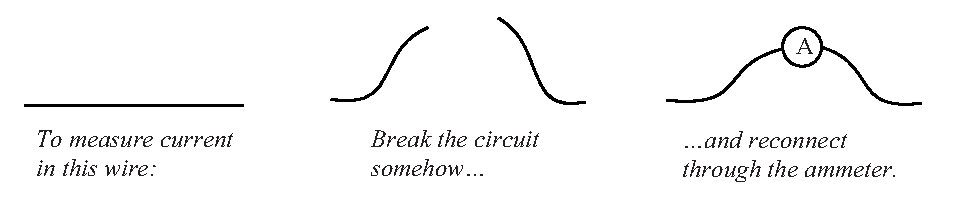
\includegraphics[height=1.5in]{electric_circuits/how_to_measure_current.eps}
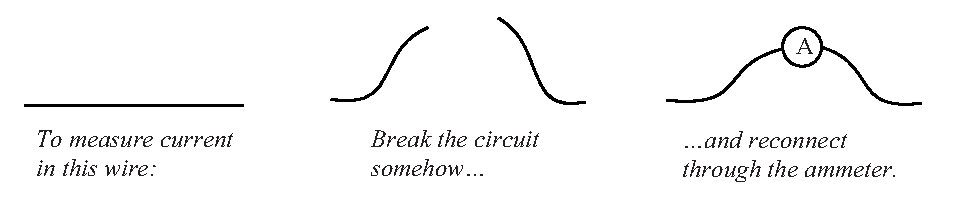
\includegraphics[width=0.8\textwidth]{electric_circuits/how_to_measure_current.eps}
\end{center}
\vspace{-0.1in}

Your DMM can also measure the potential difference, in volts between any two points in the circuit.  For this measurement, keep your circuit intact, and simply touch the two leads of the DMM to the two places in the circuit you want to measure between.

\begin{newboxed}
\textbf{For all parts of this lab, keep your power supplies set to a voltage of 3.0 volts, and use the 10A or 20A range of your DMM for measuring currents.  Otherwise we'll blow out lots of bulbs and fuses.}
\end{newboxed}

\vspace{0.1 in}
\textbf{Activity 1: Current and Voltage Measurements}

%\newpage
(a) The circuit below consists of a power supply, two ammeters, and a single light bulb.  For the following circuit, predict which of the two ammeters will measure the larger current.  (Or will they be the same?)

\begin{wrapfigure}[1]{l}{0.3\textwidth}
    \vspace{-0.4 in}
    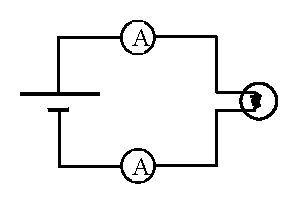
\includegraphics[width=0.3\textwidth]{electric_circuits/circ_diag1.eps}
\end{wrapfigure}

\vspace{0.2 in}
Prediction:
\vspace{1.2 in}

%\newpage
\pagebreak
(b) Build the circuit above, using your two DMMs to measure the current $I$ that flows at the two points in the circuit shown.  Record your measurements.  Was your prediction correct?
\vspace{1 in}

(c) Remove one of your two DMMs from the circuit, and use it to measure some voltage differences in the circuit as shown.  Hold the black lead at point a, and move the red lead to b, c, and d, recording the results.

\begin{wrapfigure}[2]{r}{0.35\textwidth}
    \vspace{-0.5 in}
    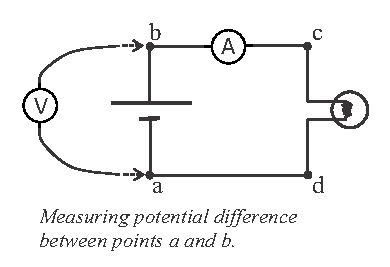
\includegraphics[width=0.35\textwidth]{electric_circuits/circ_diag2.eps}
\end{wrapfigure}

\vspace{0.3 in}
\hspace{0.5 in} $\Delta V_{ab} = $ \par
\hspace{0.5 in} $\Delta V_{ac} = $ \par
\hspace{0.5 in} $\Delta V_{ad} = $ \par
\vspace{0.6 in}

(d)  Predict the voltage difference between the two points c and d in the circuit above.  Test your prediction with a measurement.  Do they agree? \par
\hspace{0.5 in} Prediction:   $\Delta V_{cd} = $ \par
\vspace{0.2 in}
\hspace{0.5 in} Measurement:   $\Delta V_{cd} = $ \par
\vspace{0.3 in}
(e) How big is the voltage difference between the two ends of a typical wire in your circuit?
\vspace{0.6 in}



(f) How big is the voltage difference across your ammeter?  
\vspace{0.6 in}



(g) Is it reasonable to approximate either or both of the voltage differences in (e) and (f) as zero?
\vspace{0.6 in}



\textbf{Activity 2: Two Light Bulbs in Parallel}

(a) The figure below shows a circuit with a second bulb added.  These bulbs are connected ``in parallel.''  In the drawing shown, is the ammeter measuring current through just one of the lightbulbs, or through both of the lightbulbs?
\vspace{-0.1in}
\begin{flushright}
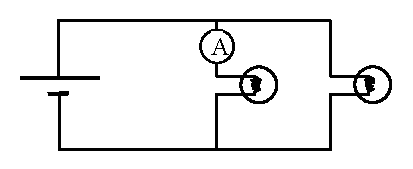
\includegraphics[width=0.4\textwidth]{electric_circuits/circ_diag3.eps}
\end{flushright}
\vspace{-0.1in}


(b) Make a prediction: If you add the second light bulb to your circuit as shown, will the current in the first light bulb increase, decrease, or stay about the same?  Build the circuit and test your prediction. \par
\hspace{0.5 in} Prediction:   \par
\vspace{0.2 in}
\hspace{0.5 in} Measurement:  \par
\vspace{0.3 in}

(c)  In the circuit you have just built, how much current is flowing from the power supply?  Make a prediction, and use a second ammeter to test your prediction. \par
\hspace{0.5 in} Prediction:   \par
\vspace{0.2 in}
\hspace{0.5 in} Measurement:  \par
\vspace{0.3 in}

\begin{center}
\framebox[1.05\width]{\textit{This is a good time to check with your instructor to be sure your measurements are on the right track.}} \par
\end{center}

%\textit{This is a good time to check with your instructor to be sure your measurements are on the right track.} \par

(d) What is the voltage difference across each of the two light bulbs in the circuit above?  Use one of your DMMs as a voltmeter to test your prediction. \par
\hspace{0.5 in} Prediction:   \par
\vspace{0.2 in}
\hspace{0.5 in} Measurement:  \par
\vspace{0.3 in}

(e) Here's a neat way to visualize electric potential, using an analogy with gravitational potential energy.  For the simple circuit that you made in activity one, imagine the circuit drawn on a piece of paper shaped like a loop, with the paper folded so that height above the table corresponds to electric potential as shown below.
\begin{center}
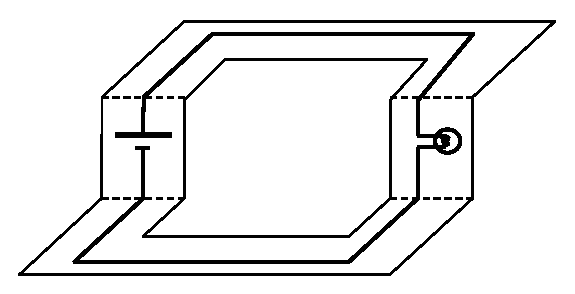
\includegraphics[width=0.5\textwidth]{electric_circuits/how_to_fold.eps}
\end{center}
\vspace{-0.1in}

On the last pages of this lab are some big circuit diagrams for you to cut out.  First, find the diagram of the circuit with two light bulbs, and use scissors to cut it into a shape with two loops.  Then fold your paper so that the height above the table corresponds to changes in potential energy.  Discuss your figure with your instructor.  Yes, you REALLY have to do this! 
\vspace{0.2 in}

(f) Is your power supply acting more like a source of fixed current, or a source of fixed voltage?  (What changes and what stays the same when you connect one or two bulbs to your power supply?) Explain.
\answerspace{0.6 in}


\pagebreak[2]
\textbf{Activity 3: Two Light Bulbs in Series} \par

(a) The circuit below shows two light bulbs connected to the power supply in series.  Make predictions for the current in each of the bulbs, and the voltage difference across each bulb.  Then build the circuit and test your predictions with measurements.  \par

\begin{wrapfigure}[1]{r}{0.3\textwidth}
    \vspace{-1.1 in}
    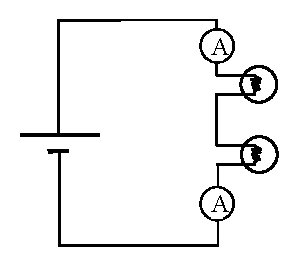
\includegraphics[width=0.3\textwidth]{electric_circuits/circ_diag4.eps}
\end{wrapfigure}

\vspace{0.1 in}
\renewcommand{\arraystretch}{1.6}
\hspace*{0.5in}
\begin{tabular}{l l}
Predictions: \hspace{0.5in} & Measurements: \\
$I_1 =$ & $I_1 =$ \\
$\Delta V_1 =$ & $\Delta V_1 =$ \\
$I_2 =$ & $I_2 =$ \\
$\Delta V_2 =$ & $\Delta V_2 =$ \\
\end{tabular}
\renewcommand{\arraystretch}{1.0}
\vspace{0.3in}

(b)  Cut out the picture of this circuit from the final pages of your lab, and fold it so that height above the table represents electric potential.  Discuss your figure with your instructor. 

\textit{(A quick note for those who have studied circuits before:  You may have expected the current in each of the bulbs to be exactly half of the current through a bulb in the previous exercises.  That would be true if the bulbs were regular resistors.  But in fact, the ``resistance'' of these bulbs changes as they get hot, so they don't obey Ohm's law.)}

\textbf{Activity 4: Bulbs in series and in parallel} \par
\nopagebreak
(a) The circuit shown below includes light bulbs in series and in parallel with each other.  Predict the values of the currents and voltage differences for each bulb, and then test your predictions.  Which bulb or bulbs will be brightest? \par

\begin{wrapfigure}[1]{r}{0.4\textwidth}
    \vspace{-1.0 in}
    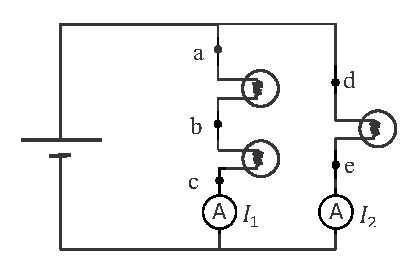
\includegraphics[width=0.4\textwidth]{electric_circuits/circ_diag5.eps}
\end{wrapfigure}

\vspace{0.1 in}
\renewcommand{\arraystretch}{1.6}
\hspace*{0.5in}
\begin{tabular}{l l}
Predictions: \hspace{0.7in} & Measurements: \\
$I_1 =$ & $I_1 =$ \\
$I_2 =$ & $I_2 =$ \\
$\Delta V_{ab} =$ & $\Delta V_{ab} =$ \\
$\Delta V_{bc} =$ & $\Delta V_{bc} =$ \\
$\Delta V_{de} =$ & $\Delta V_{de} =$ \\
Brightest bulb: & Brightest bulb: \\
\end{tabular}
\renewcommand{\arraystretch}{1.0}
\vspace{0.3in}

(b) What is the relationship between bulb brightness and current through the bulb?
\vspace{0.5 in}

(c) What is the relationship between bulb brightness and voltage difference across the bulb?
\vspace{0.5 in}

\newpage
\begin{samepage} %This samepage command had no effect whatsoever.  How do I make this behave, without hardcoding a page break?
(d) If we define the electric potential at the negative terminal of the power supply to be at $V=0$ Volts, what is the potential at each of the points a, b, c, d, and e in the circuit drawing above?  
\vspace*{0.6 in}
\end{samepage}

\textbf{Homework}

Problem 1: Consider the following circuit:

\begin{center}
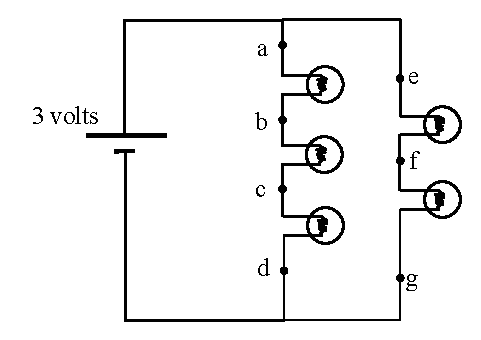
\includegraphics[width=0.45\textwidth]{electric_circuits/circ_diag6.eps}
\end{center}
\vspace{-0.1in}

(a) If we define the electric potential at the negative terminal of the power supply to be at $V=0$ Volts, what is the potential at each of the points a, b, c, d, e, f, and g?  
\vspace{0.7 in}

(b) Rank from smallest to largest the current at each of the lettered points in the circuit.   (You can write ``$I_c<I_a=I_f<I_e…$'' or something like that.) 
\vspace{0.7 in}

(c) Which bulb or bulbs will be brightest?  Which bulb or bulbs will be least bright?
\vspace{1.7 in}

\textit{(Problem 2 is on the next page.  Keep going....)}
\newpage
Problem 2: Consider the following circuit:

\begin{center}
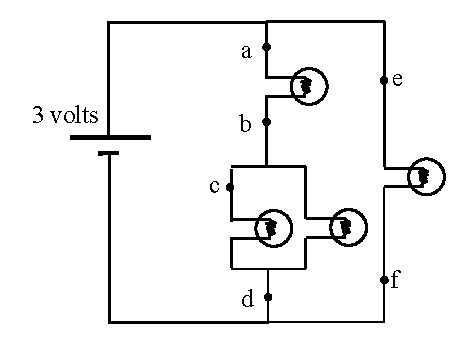
\includegraphics[width=0.5\textwidth]{electric_circuits/circ_diag7.eps}
\end{center}
\vspace{-0.1in}

(a) Which is greater, $\Delta V_{ab}$ or  $\Delta V_{ef}$?  Why?
\vspace{0.6 in}

(b) Which bulb is brighter, the one between a and b, or the one between e and f?  Why?
\vspace{0.6 in}

(c) Which is greater, $I_a$ or $I_e$?  Why?
\vspace{0.6 in}

(d) Which is greater, $I_c$ or $I_b$? Why?
\vspace{0.6 in}

(e) Which is greater, $\Delta V_{ab}$ or  $\Delta V_{cd}$? Why?
\vspace{0.6 in}

(f) Cut out the circuit on the last page of this lab, and fold it so that height above the table represents electric potential.  Now that you have folded it, are there any answers above you’d like to change?  Bring your folded paper to class, and be prepared to discuss your figure with your instructor.
\vspace{0.6 in}

\cleardoublepage %force this cutout page to be on the right hand side.
\begin{center}
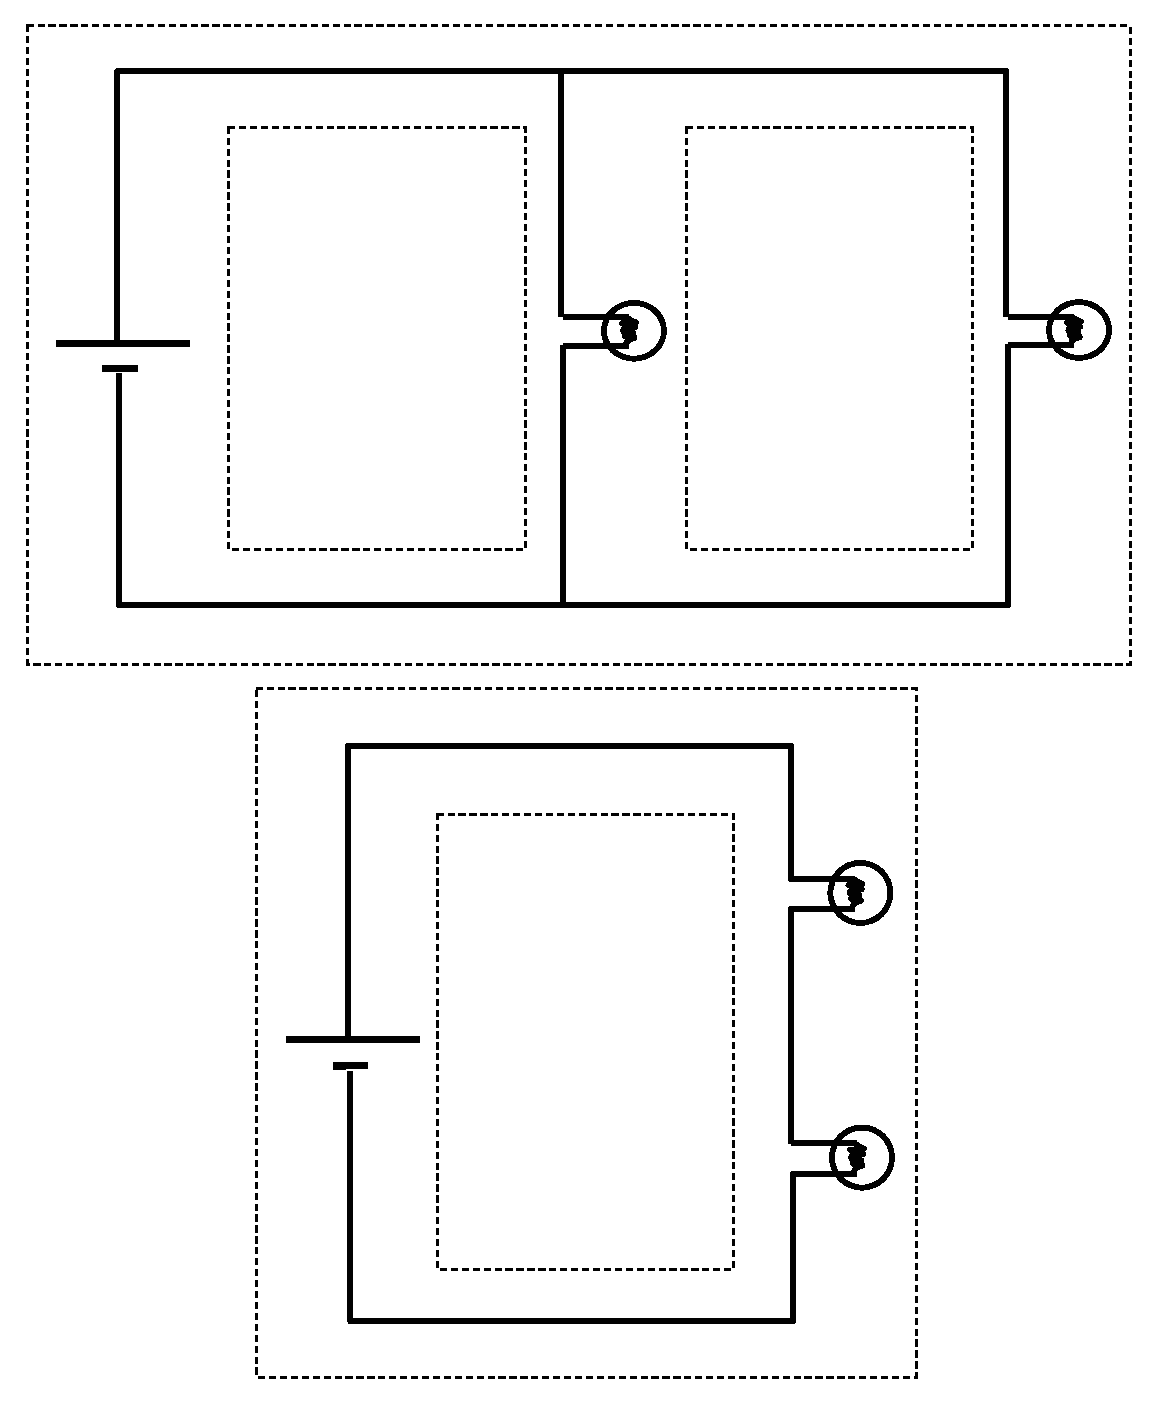
\includegraphics[width=0.95\textwidth]{electric_circuits/cutout_page1.eps}
\end{center}

\newpage
[This page left intentionally blank, at least mostly.]
\newpage

\begin{center}
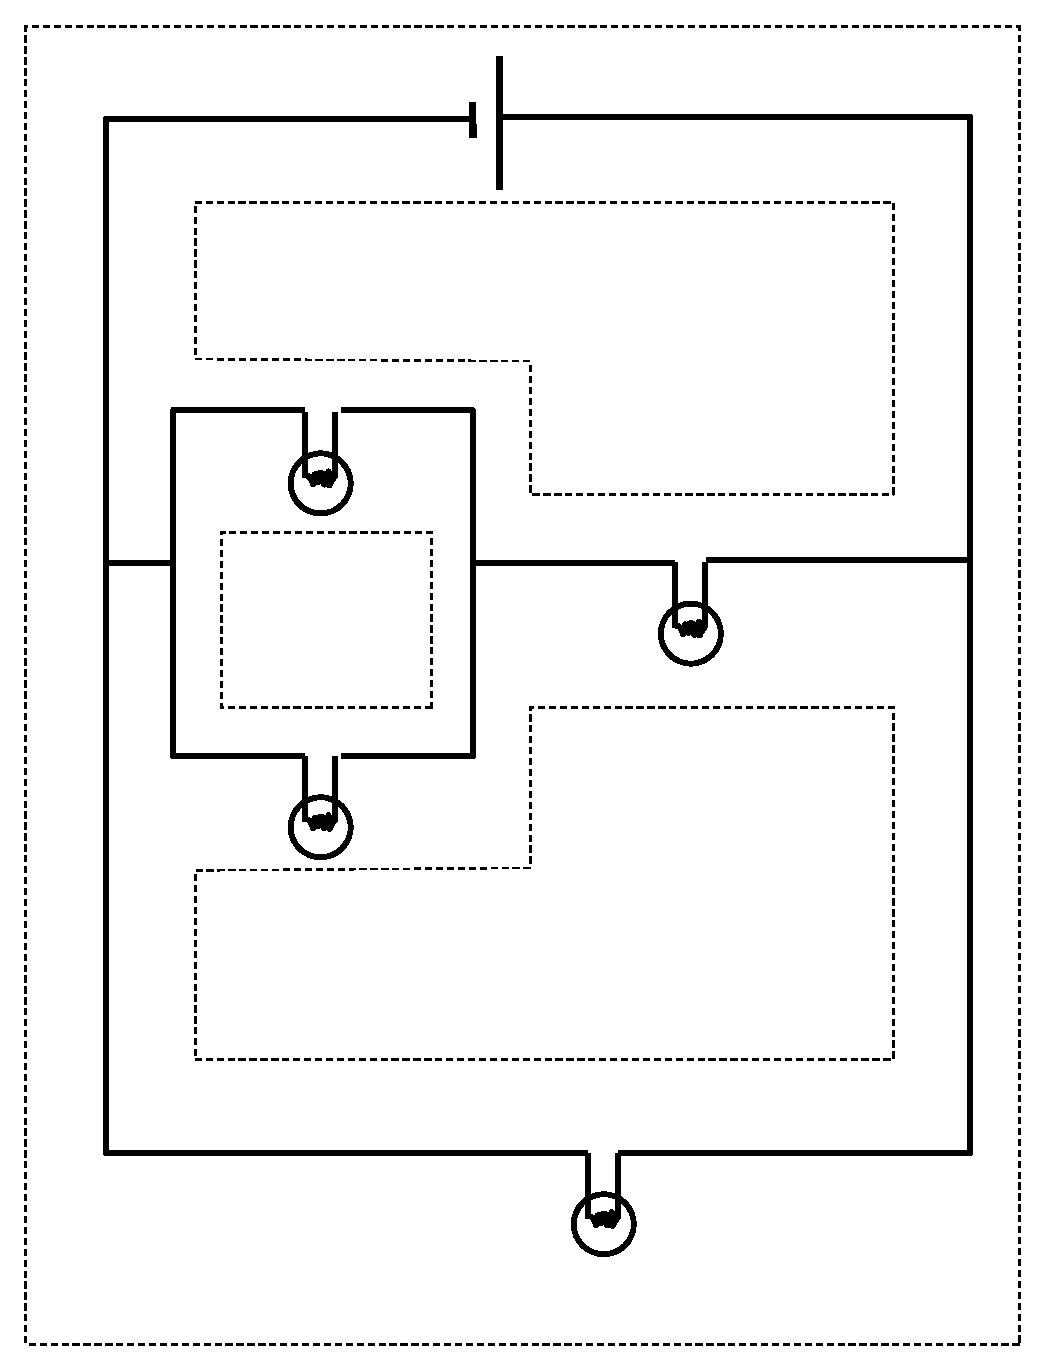
\includegraphics[width=0.95\textwidth]{electric_circuits/cutout_page2.eps}
\cleardoublepage

\end{center}


